\section{Results}\label{section:eval-results}

% Commands to edit stats which might change later. 

% demographic questions
\newcommand{\participantsCount}{23}
\newcommand{\participantsMale}{21}
\newcommand{\participantsAge}{23}

% model viewer statistical facts
\newcommand{\evalExpMvAvgPoses}{2.83}
\newcommand{\evalExpMvStdPoses}{1.94}
\newcommand{\evalExpMvParticipants}{\participantsCount}

% avg lp experiments
\newcommand{\kammAvgHits}{36.23/60}
\newcommand{\kammAvgStd}{6.87/60}
\newcommand{\youngAvgHits}{0.85}
\newcommand{\youngAvgStd}{-}
\newcommand{\oursAvgHits}{26.13/30}
\newcommand{\oursAvgStd}{5.52/30}

% model viewer sus scores
\newcommand{\evalExpMvSusScore}{83.04}
\newcommand{\evalExpMvSusGrade}{B}
\newcommand{\evalExpMvSusAdj}{\enquote{Good}}

% model viewer sus scores
\newcommand{\evalExpLpSusScore}{91.41}
\newcommand{\evalExpLpSusGrade}{A}
\newcommand{\evalExpLpSusAdj}{\enquote{Excellent}}

% model viewer sus scores
\newcommand{\evalExpVkSusScore}{71.63}
\newcommand{\evalExpVkSusGrade}{C}
\newcommand{\evalExpVkSusAdj}{\enquote{Ok}}


% Calculations
\newcommand{\participantsFemale}{\pgfmathparse{\participantsCount - \participantsMale}\pgfmathprintnumber[fixed, precision=2]{\pgfmathresult}}%chktex 8 chktex 1

% First try in performing a T-Test. TODO: Check with michael
% \pgfmathparse{10/6.5}\pgfmathprintnumber[fixed, precision=2]{\pgfmathresult}

% This evaluation of the preliminary questions is pretty WIP.

\participantsCount{} persons participated in the evaluation. \participantsFemale{} stated, they identify as female and \participantsMale{} identify as male. The average age is \participantsAge{} years. 

\begin{table}[H]
  \centering
  \begin{subtable}{.5\linewidth}
    \footnotesize
    \centering
    \begin{tabular}{l c c}
      \toprule
      Degree & Count & Percentage\\
      \midrule
      High school degree & 13 &	56.52\% \\
      Bachelor's degree (BA) & 6 & 26.09\% \\
      Diploma's degree (Dipl.) & 1 & 4.35\% \\
      Master's degree (MA) & 2 & 8.70\% \\
      Approbation	& 1 &	4.35\% \\
      \bottomrule
    \end{tabular}
    \caption{The answers to question A3: \enquote{What is the highest degree or level of school you have completed?}}\label{tab:sus-degree}
  \end{subtable}%
  \begin{subtable}{.5\linewidth}
    \footnotesize
    \centering
    \begin{tabular}{l c c}
      \toprule
      Discipline & Count & Percentage\\
      \midrule
      Informatics & 7 & 30.43\% \\
      Physics & 2 & 8.70\% \\
      Automation and Robotics & 1 & 4.35\% \\
      Book Science & 1 & 4.35\% \\
      Chemistry & 1 & 4.35\% \\
      Computational Biology & 1 & 4.35\% \\
      Economics & 1 & 4.35\% \\
      Electrical Engineering & 1 & 4.35\% \\
      Law & 1 & 4.35\% \\
      Medicine & 1 & 4.35\% \\
      Musicology & 1 & 4.35\% \\
      Pharmacy & 1 & 4.35\% \\
      Public Service & 1 & 4.35\% \\
      Statistics & 1 & 4.35\% \\
      Technical Engineering & 1 & 4.35\% \\
      Technology Management & 1 & 4.35\% \\
      \bottomrule
      \end{tabular}
      \caption{The answers to question A4: \enquote{What is your main discipline?}}\label{tab:sus-discipline}
  \end{subtable}
  \caption[Degree and discipline of participants]{Highest degree (question A3) and main discipline (question A4) of the participants.}\label{tab:sus-d}
\end{table}

The main disciplines and degrees are shown in Table~\ref{tab:sus-d}. As seen in Table~\ref{tab:sus-degree}, the highest degree of half of the participants was a high school degree or equivalent. Table~\ref{tab:sus-discipline} shows that the main discipline is quite spread amongst different disciplines.

\begin{figure}[H]
  \centering
  \begin{subfigure}{.48\linewidth}%
    \centering
    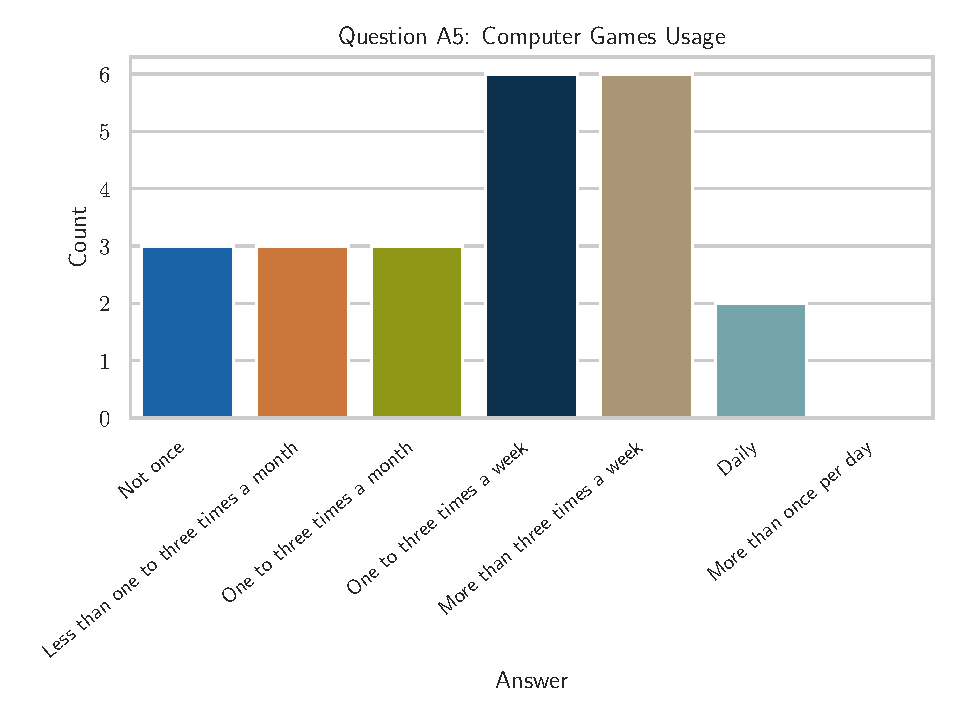
\includegraphics[width=\linewidth]{figures/evaluation/res_demo_q8_s3.pdf}
    \caption{The answers to the question A5: \enquote{Please rate how much you used computer games in the last six months.}}\label{fig:res-demo-q8-s3}
  \end{subfigure}%
  \hspace{0.03\linewidth}
  \begin{subfigure}{.48\linewidth}%
    \centering
    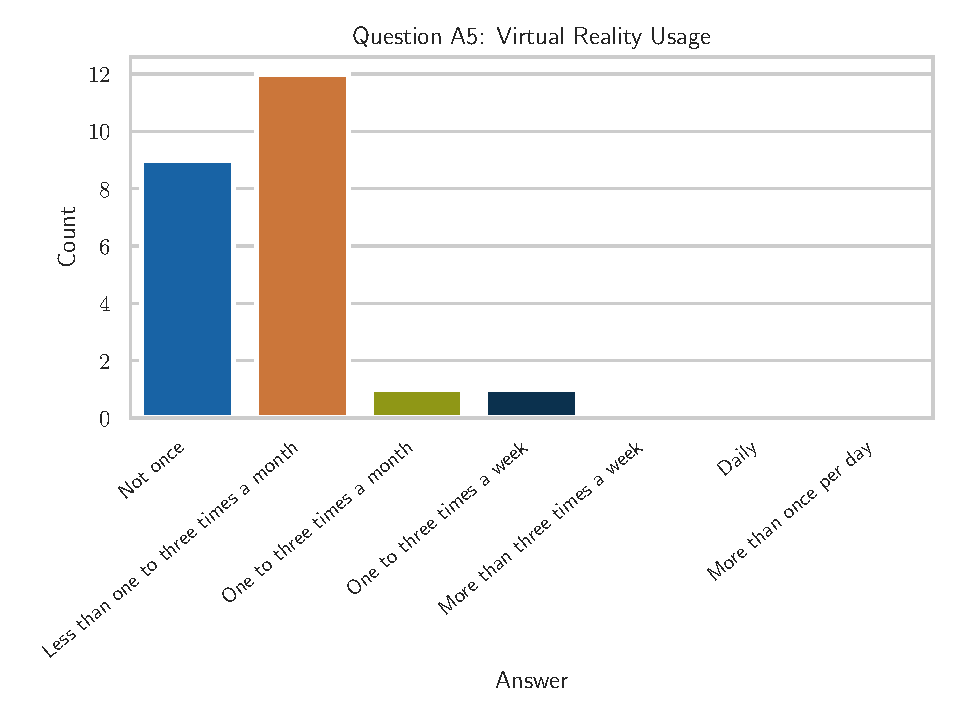
\includegraphics[width=\linewidth]{figures/evaluation/res_demo_q8_s4.pdf}
    \caption{The answers to the question A5: \enquote{Please rate how much you used virtual reality headsets in the last six months.}}\label{fig:res-demo-q8-s4}
  \end{subfigure}%
  \caption[Computer games and virtual reality headset usage]{The results of the question A5 about the computer games and virtual reality headset usage.}\label{fig:res-demo-q8}
\end{figure}

All participants (100.00\%) used their smartphone multiple times a day during the last six months. Most participants (78.26\%) used their computer for work or studies more than once per day during the last six months. 17.39\% state that they used it daily and only one participant used his computer one to three times a week for work or studies during the last six months. As seen in Figure~\ref{fig:res-demo-q8-s3}, most participants (60.87\%) played computer games more than three times a month during the last six months. Figure~\ref{fig:res-demo-q8-s4} shows that most participants (91.30\%) used \ac{VR} less than once per month during the last six months. A huge portion (39.13\%) did not use \ac{VR} at all in the last six moths.

\begin{figure}[H]
  \centering
  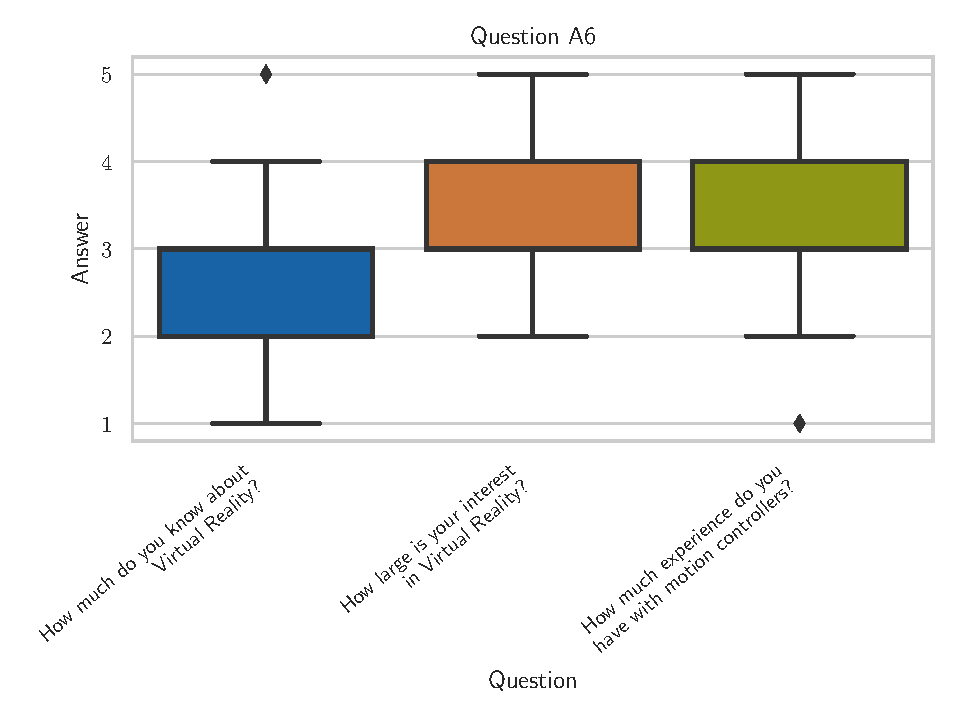
\includegraphics[width=10cm]{figures/evaluation/res_demo_q9.pdf}
  \caption[VR experience of the participants]{The results of the question A6 about the experience of the participants with \ac{VR}. The questions are rated with values ranging from one (\enquote{none}) to five (\enquote{a lot}).}\label{fig:res-demo-q9}
\end{figure}

The participants were asked three questions regarding their experience with \ac{VR} which could be answered with values ranging from one (\enquote{none}) to five (\enquote{a lot}). The first questions asked about the knowledge the user had about \ac{VR}. As can be seen in the box plots\footnote{The boxes indicate the range from the \nth{25} to the \nth{75} percentile. The bars outside the box (\enquote{whiskers}) indicate the \nth{90} and \nth{10} percentile. The median (\nth{50} percentile) is marked by the line in the center. Outliers are marked with diamond shapes.} in Figure~\ref{fig:res-demo-q9}, the general knowledge about \ac{VR} seems to be rather low (Mean: 2.83; \ac{STD}: 1.03). The second question asked about the interest in \ac{VR}, to which not one participant answered with the value one (Mean: 3.48; \ac{STD}: 0.99). The last question asked about the experience with motion controllers. It was explicitly mentioned that the Wii remote counts as motion controller, which might be the reason for the average, which is higher than the one from the first question (Mean: 3.30; \ac{STD}: 1.22).
%The evaluation was conducted during different times of the day. does say nothing


\subsection{Model Viewer}\label{section:eval-res-mv}

The model viewer experiment, described in Section~\ref{subsection:model-viewer}, allows users to view a \ac{3D} model from different angles. To benchmark extensive usage, a second model instance in another color (the target) is spawned after starting the task. Since in the current implementation, the model cannot be rotated upside down (as mentioned in Section~\ref{subsection:topic-data}), the target is spawned with random reachable orientations.
As soon as the task is started, the user has 30 seconds to match as many orientations as possible. Similar to the implementation by \citeauthor{Katzakis.2010}, the target is rotated to a new random orientation, after one orientation was matched~\cite[140]{Katzakis.2010}.
Because it is hard to match the rotation exactly on all three axes, it is enough to pose the model in a similar orientation to the target. A similar pose is reached, when the smallest angle between the two rotations is less than 20 radians.

\begin{figure}[H]
  \centering
  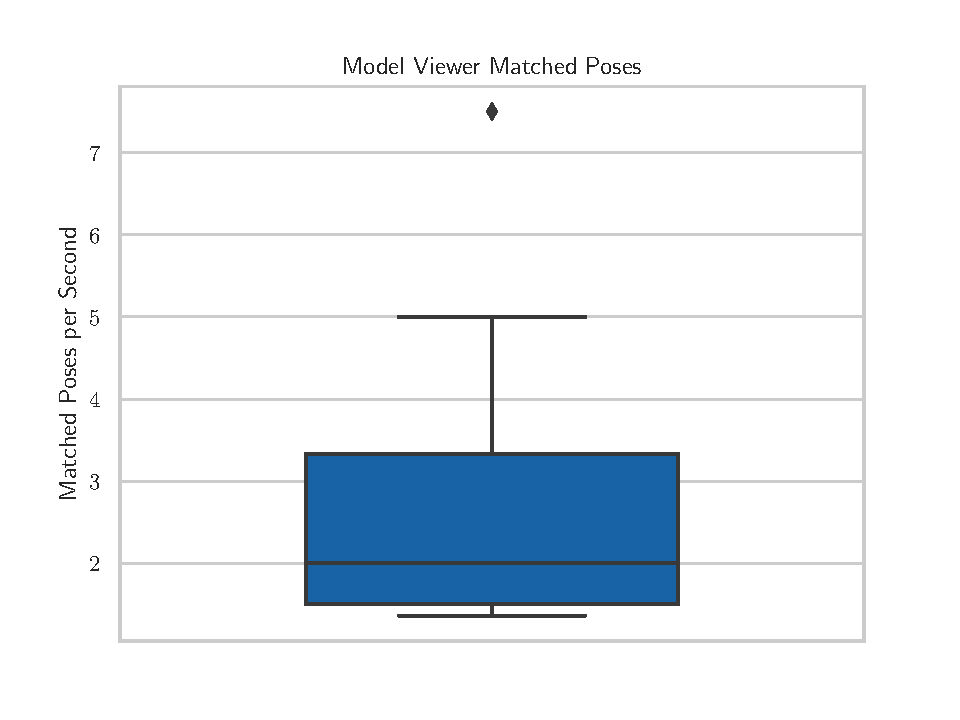
\includegraphics[width=10cm]{figures/evaluation/eval_exp_mv.pdf}
  \caption[Model viewer experiment results]{The time in seconds it took to match a correct pose in the model viewer experiment.}\label{fig:eval-exp-mv}
\end{figure}

% TODO: T-Test:
%\pgfmathparse{(\evalExpMvAvgPoses-6.5)/(\evalExpMvStdPoses/sqrt(\evalExpMvParticipants))}\pgfmathprintnumber[fixed, precision=2]{\pgfmathresult} 
% chktex 1
As seen in Figure~\ref{fig:eval-exp-mv}, the average time it took to match a correct poses is roughly \evalExpMvAvgPoses{} seconds. \citeauthor{Katzakis.2010} tracked the time it takes to match a pre-defined pose with a Smartphone, a mouse and a touch panel. The lowest time in average to match one pose, 6.5 seconds, was achieved using the Smartphone as input device~\cite[140]{Katzakis.2010}. The average time to match a pose of the model viewer (\evalExpMvAvgPoses{} seconds) experiment presented in Chapter~\ref{section:eval-res-mv} is lower than the average of the evaluation of \citeauthor{Katzakis.2010} (6.5 seconds). This can be due to the fact that users never had to turn the smartphone completely upside down, since rotations were chosen to be always upside up, because of the previously mentioned limitation. Another advantage of the presented implementation is, that the target and the controlled model are not displayed in two separate locations like in {\citetitle{Katzakis.2010}}, but rather with the same origin in the same coordinate space, which makes it easier to see the difference between both rotations~\cite[140]{Katzakis.2010}. Also the fact that a skeleton model instead of a multi-colored cube was used, could play a role. 

\begin{figure}[H]
  \centering
  \begin{subfigure}{.48\linewidth}%
    \centering
    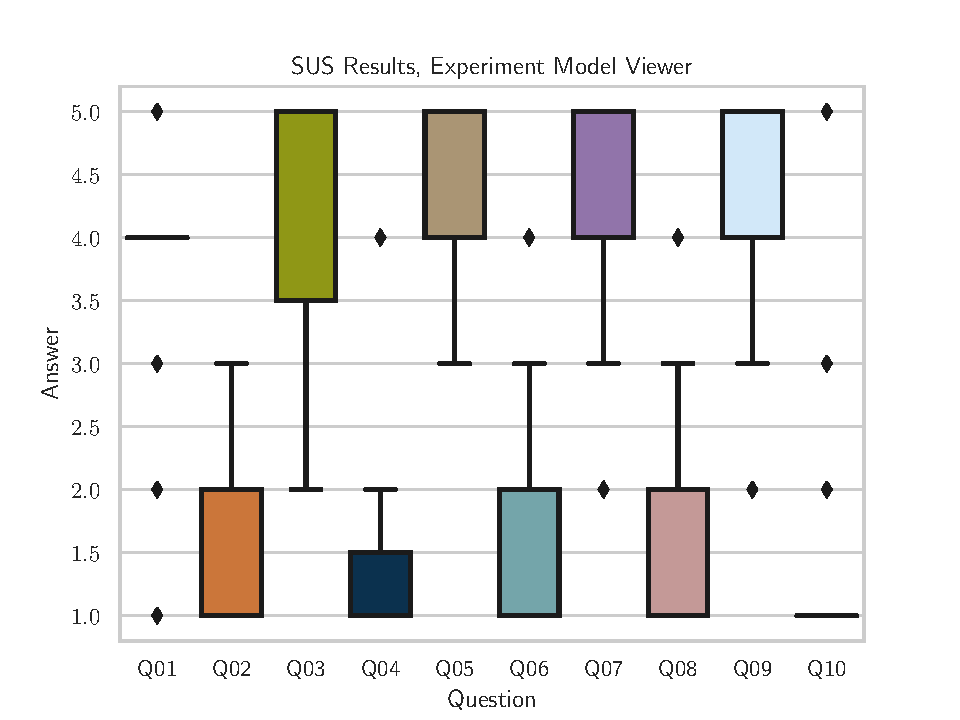
\includegraphics[width=\linewidth]{figures/evaluation/res_exp_mv.pdf}
    \caption{The results of question one to ten.}\label{fig:res-exp-mv}
  \end{subfigure}%
  \hspace{0.03\linewidth}%
  \begin{subfigure}{.48\linewidth}%
    \centering
    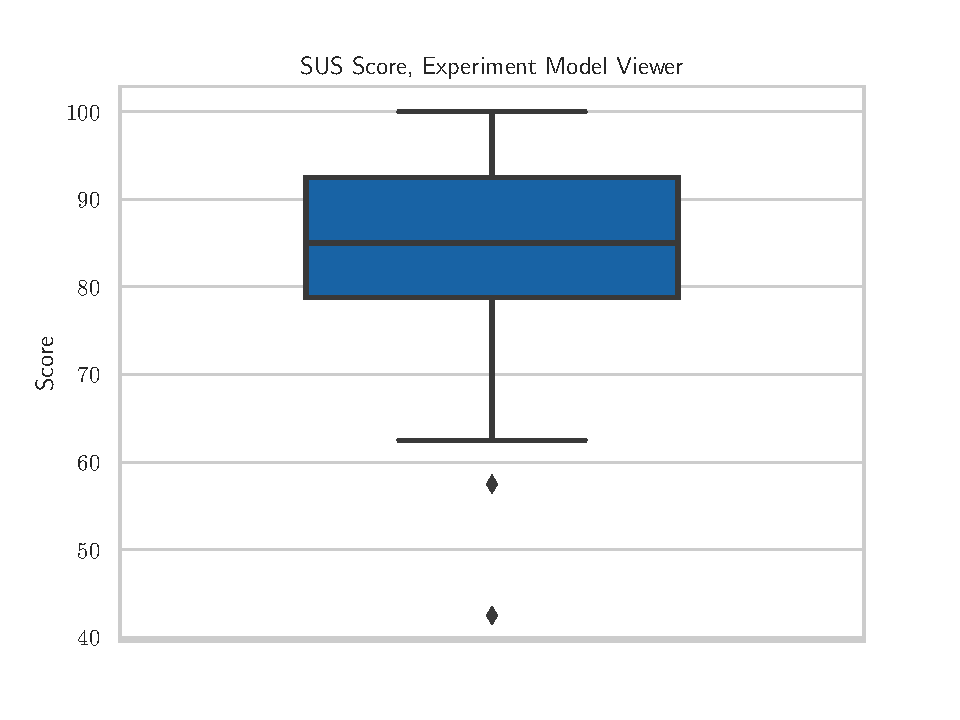
\includegraphics[width=\linewidth]{figures/evaluation/score_exp_mv.pdf}
    \caption{The overall \ac{SUS} score.}\label{fig:score-exp-mv}
  \end{subfigure}%
  \caption[User study results of the model viewer experiment]{The results of the \ac{SUS} user study for the model viewer.}\label{fig:exp-mv-stats}
\end{figure}

Also the \ac{SUS} study results indicate a useable implementation, as seen in Figure~\ref{fig:exp-mv-stats}. A score of \evalExpMvSusScore{} is considered \evalExpMvSusAdj{} and mapped to the grade \evalExpMvSusGrade, according to \citeauthor{Bangor.2009}~\cite[120\psq]{Bangor.2009}.


% TODO:
Further, many users made comments about the experiment:

\begin{itemize}
  \item lul
\end{itemize}




\subsection{Laser Pointer}\label{section:eval-res-lp}

Section~\ref{subsection:laser-pointer} introduces the laser pointer experiment. To test the performance of participants using this interaction, three cubes (the targets) are spawned at random locations in front of the user. The cubes are always spawned in sight of the user so that he does not has to actively look for the targets. The participant has to select as much cubes as possible in 30 seconds. He was told to be as fast and especially as accurate as possible, since miss-hits are counted. 

To trigger a selection, the user has to touch the smartphone display. This counts as a click. If no cube was selected, a miss is counted. The total selection (click) count is the sum of hits and miss-clicks. If one cube was hit, another one is spawned, so that always three cubes are visible. This is important, because the user can plan to hit the next target while currently aiming for the current one. Otherwise the task would test the users reaction time, which is not desired. 

\begin{figure}[H]
  \centering
  \begin{subfigure}{.48\linewidth}%
    \centering
    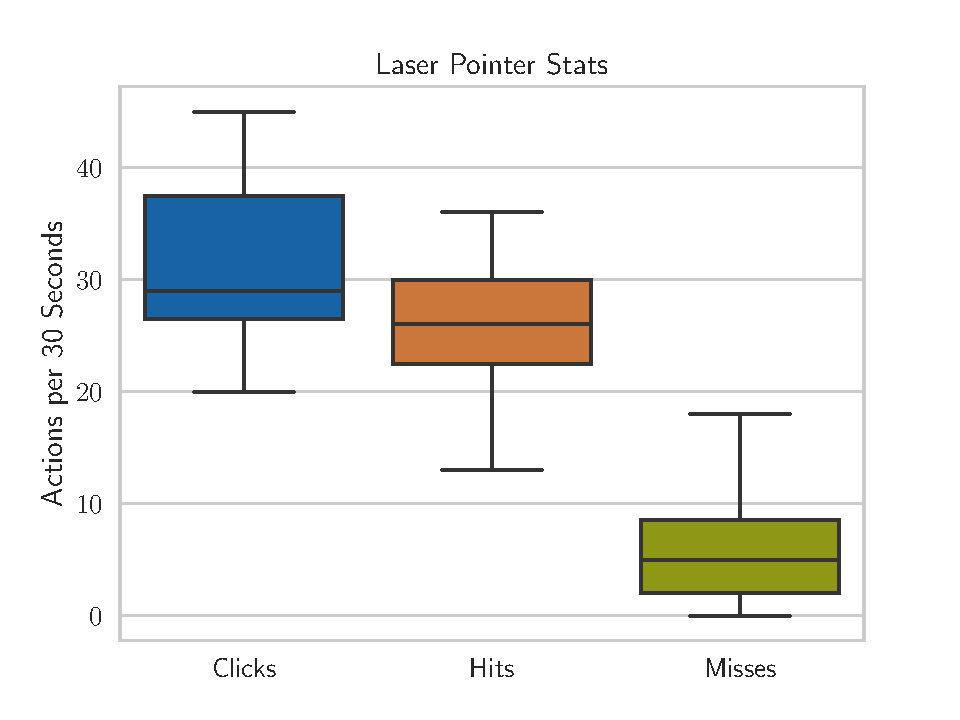
\includegraphics[width=\linewidth]{figures/evaluation/eval_exp_lp.pdf}
    \caption{The count of clicks, hits and misses per 30 seconds. Clicks are the sum of hits and misses.}\label{fig:eval-exp-lp}
  \end{subfigure}%
  \hspace{0.02\linewidth}%
  \begin{subfigure}{.48\linewidth}%
    \centering
    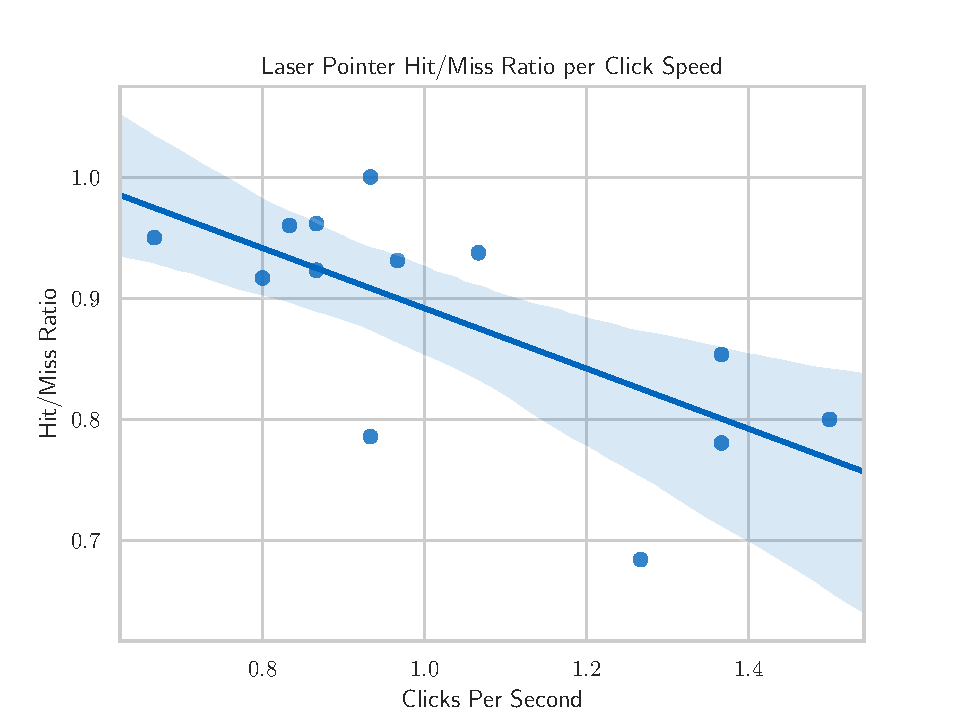
\includegraphics[width=\linewidth]{figures/evaluation/eval_exp_lp_ratio_scatter.pdf}
    \caption{The Hit/Miss ratio per click speed.}\label{fig:eval-exp-lp-ratio-scatter} %The line visualizes the linear regression with a 95\% confidence interval.
  \end{subfigure}%
  \caption[Laser pointer experiment results]{The results of the laser pointer experiment.}\label{fig:exp-lp-eval}
\end{figure}

Figure~\ref{fig:eval-exp-lp} visualizes the total click count (Mean: 31.83; \ac{STD}: 6.89), the actual hit count (Mean: 26.13; \ac{STD}: 5.52) and the count of miss hits (Mean: 5.70; \ac{STD}: 4.37) per 30 seconds. Participants were able to successfully point to and select objects with a speed of nearly one click per second. As seen in Figure~\ref{fig:eval-exp-lp-ratio-scatter} the hit/miss ratio is very high for slightly lower speeds but decreases fast with higher click speeds.

The performance of this experiment is hard to compare with other implementations, without a standardized experiment setup. For example the size, shape, position and distance of the targets but also the spawn area and wether distracting elements are present or not, varies between different task evaluations of other research. However a comparison should still give a rough estimate wether the performance is similar, much better or really bad. Often the hit count is measured in different time intervals. To compare the results, the average hit count per second is calculated.

\citeauthor{Kamm.2018} tested his implementation in a similar \ac{VR} scenario with a wrist band as input device. To compare his implementation, he also tested a laser pointer approach using a \ac{VR} motion controller~\cite[39]{Kamm.2018}. A major difference to his experiment setup is, that only one target is displayed at a time. Another difference is, that the user has to rotate his head more in order to see the targets, since they are placed in a 90 degrees radius. An arrow, which always points to the next target, is displayed to prevent wasting time while searching for the next one. Also the distance from the user to the targets is randomized~\cite[45]{Kamm.2018}.

\citeauthor{JiYoungOh.2002} compared a real-world laser pointer for large screen interactions to a computer mouse. The application is displayed through a projector and the laser is detected by a camera. The pointer-device also has a button, which is pressed down to select an object, similar to the laser pointer implementation presented in Chapter~\ref{section:eval-res-lp}. All targets are always visible and their is a pre-determined order. Also the fact that all objects are on the same plane, makes the task similar to the one presented in this thesis~\cite[3\psq]{JiYoungOh.2002}.

\begin{table}
  \centering
    \begin{tabular}{l c c}
    \toprule
    Source & Average Hits per Second & Standard Deviation\\
    \midrule
    \cite{Kamm.2018} & \pgfmathparse{\kammAvgHits}\pgfmathprintnumber[fixed, precision=2]{\pgfmathresult} & \pgfmathparse{\kammAvgStd}\pgfmathprintnumber[fixed, precision=2]{\pgfmathresult}\\%chktex 2 
    \cite{JiYoungOh.2002} & \youngAvgHits{} & \youngAvgStd{} \\%chktex 2 21
    Chapter~\ref{section:eval-res-lp} & \pgfmathparse{\oursAvgHits}\pgfmathprintnumber[fixed, precision=2]{\pgfmathresult} & \pgfmathparse{\oursAvgStd}\pgfmathprintnumber[fixed, precision=2]{\pgfmathresult}\\
    \bottomrule
    \end{tabular}
  \caption[Comparison of laser pointer task results from other research.]{Comparison of the average hits per second from similar laser pointer experiments of other research.}\label{tab:lp-comp}
\end{table}

As seen in Table~\ref{tab:lp-comp}, the technique presented in Chapter~\ref{section:eval-res-lp} is the one with the best results. But due to the different conditions and task setups, it is not possible to draw a strong conclusion. Still, the result is similar to a real-world pointing technique, which is a good sign.

\begin{figure}[H]
  \centering
  \begin{subfigure}{.48\linewidth}%
    \centering
    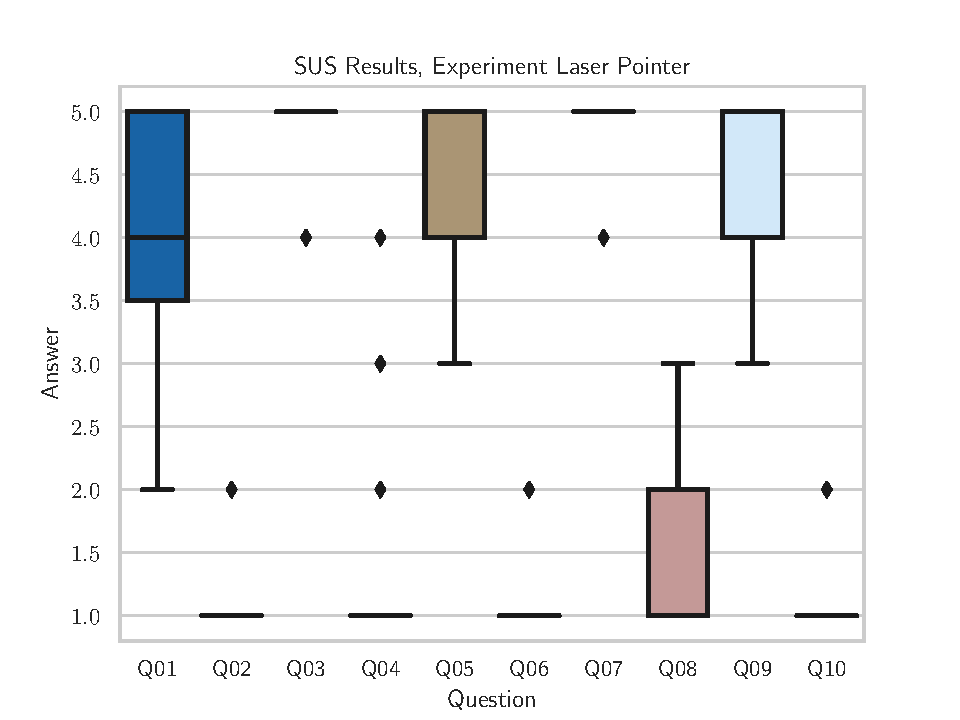
\includegraphics[width=\linewidth]{figures/evaluation/res_exp_lp.pdf}
    \caption{The results of question one to ten presented as box plots.}\label{fig:res-exp-lp}
  \end{subfigure}%
  \hspace{0.04\linewidth}%
  \begin{subfigure}{.48\linewidth}%
    \centering
    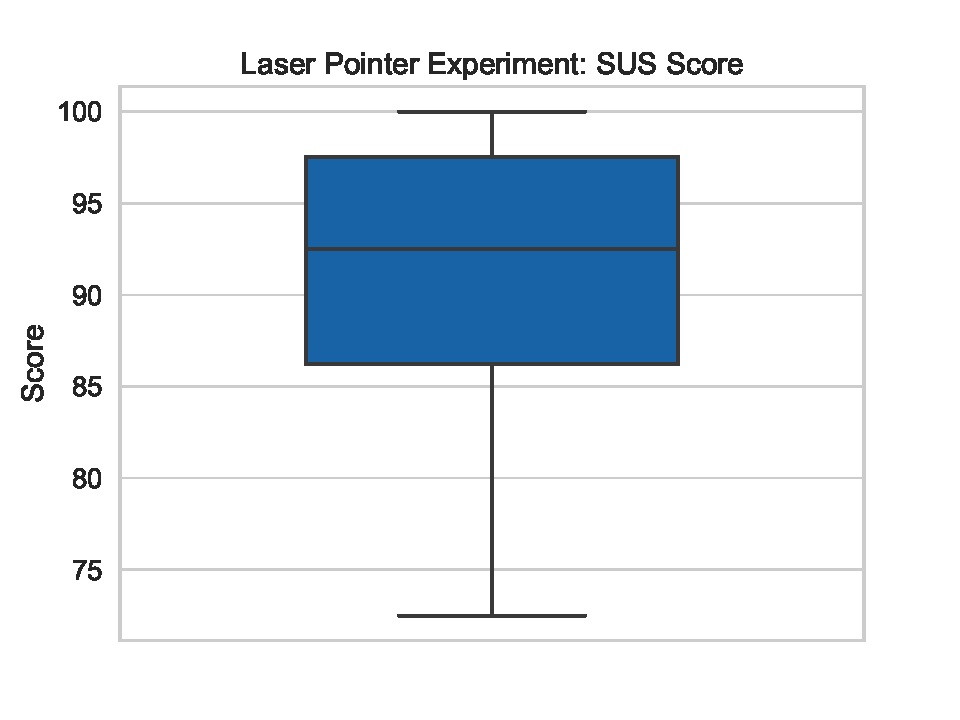
\includegraphics[width=\linewidth]{figures/evaluation/score_exp_lp.pdf}
    \caption{The overall \ac{SUS} score presented in a box plot.}\label{fig:score-exp-lp}
  \end{subfigure}%
  \caption[User study results of the laser pointer experiment]{The results of the \ac{SUS} user study for the laser pointer.}\label{fig:exp-lp-stats}
\end{figure}

However, not only the measured interaction times but also the \ac{SUS} study results indicate a useable implementation, as seen in Figure~\ref{fig:exp-lp-stats}. A score of \evalExpLpSusScore{} is considered \evalExpLpSusAdj{} and mapped to the grade \evalExpLpSusGrade{}, according to \citeauthor{Bangor.2009}~\cite[120\psq]{Bangor.2009}.


% TODO:
Further, many users made comments about the experiment:

\begin{itemize}
  \item lul
\end{itemize}




\subsection{Virtual Keyboard}\label{section:eval-res-vk}

The task for the virtual keyboard experiment, presented in Chapter~\ref{subsection:virtual-keyboard}, is to enter a text as fast as possible without mistakes. The text chosen for this task is \enquote{A quick brown fox jumps over the lazy dog}, which is commonly used when testing keyboards, typewriters or fonts because it contains all characters of the alphabet. To test the \enquote{shift}-key more than just with the first capitalized letter, also a exclamation mark is added at the end. This given text is displayed on top of the text which is currently typed with the keyboard. If a mistake was made, is has to be corrected in order to complete the task. After starting the task, a timer counts the time until the \enquote{enter}-button is pressed.

\begin{figure}[H]
  \centering
  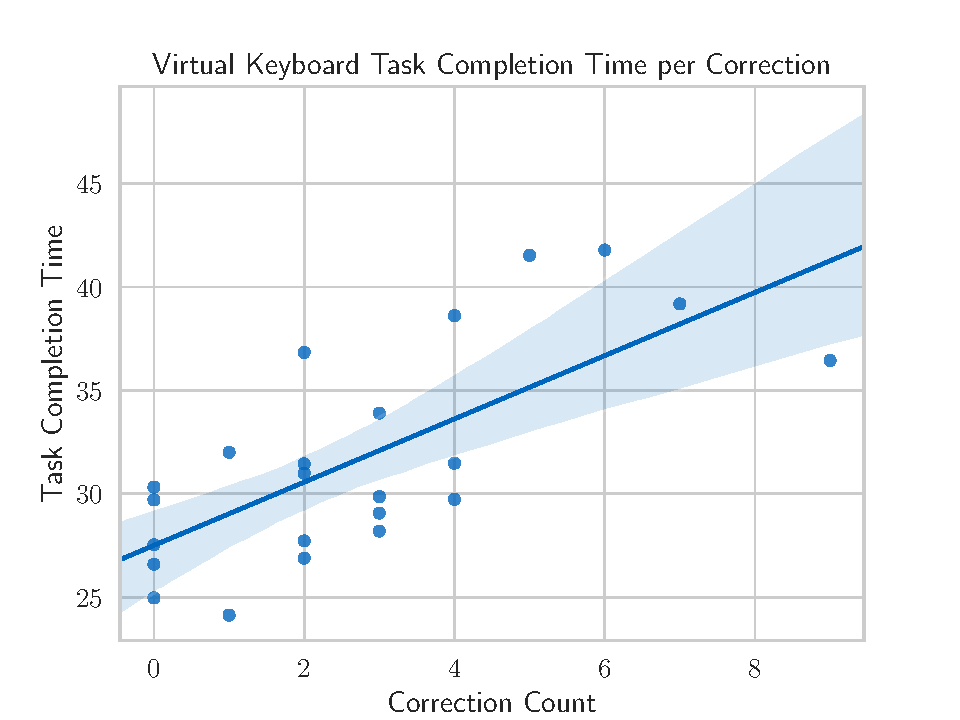
\includegraphics[width=10cm]{figures/evaluation/eval_exp_vk_ratio_scatter.pdf}
  \caption[Virtual keyboard experiment results]{The time it took to complete the virtual keyboard task per correction count. The line visualizes the linear regression with a 95\% confidence interval.}\label{fig:eval-exp-vk-ratio-scatter}
\end{figure}

The count of corrections the participants made while entering the given text has an average of 2.7 (mean: 2.74; \ac{STD}: 2.38). A correction is counted, when the user uses the \enquote{backspace}-key to remove one character. If he did not recognize his error soon enough, it is possible that in order to correct one letter, the user has to remove multiple characters which are counted as multiple \enquote{corrections}. Since the participant has to type a total of 42 characters, the average correction count to character count ratio is at 6.52\%.
Participants took 31.7 seconds in average (\ac{STD}: 5.1) to complete the task. Figure~\ref{fig:eval-exp-vk-ratio-scatter} shows that the more mistakes were made, the more time users needed to complete the task.

\begin{figure}[H]
  \centering
  \begin{subfigure}{.5\linewidth}%
    \centering
    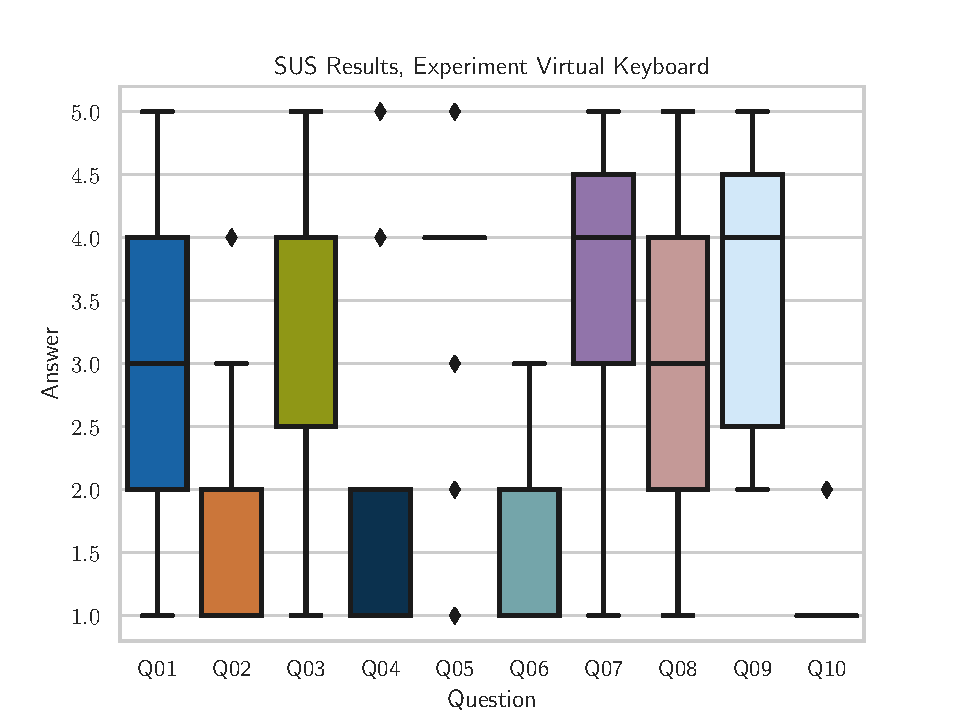
\includegraphics[width=\linewidth]{figures/evaluation/res_exp_vk.pdf}
    \caption{The results of question one to ten.}\label{fig:res-exp-vk}
  \end{subfigure}%
  \begin{subfigure}{.5\linewidth}%
    \centering
    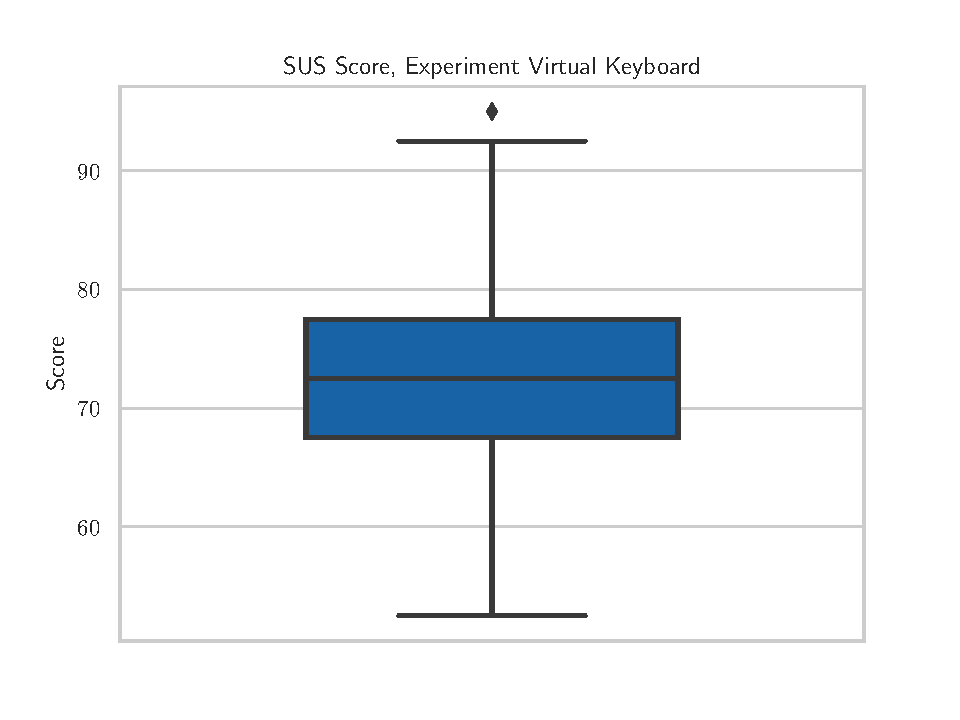
\includegraphics[width=\linewidth]{figures/evaluation/score_exp_vk.pdf}
    \caption{The overall \ac{SUS} score.}\label{fig:score-exp-vk}
  \end{subfigure}%
  \caption[User study results of the virtual keyboard experiment]{The results of the \ac{SUS} user study for the virtual keyboard.}\label{fig:exp-vk-stats}
\end{figure}

The \ac{SUS} score for this experiment, shown in Figure~\ref{fig:exp-mv-stats}, is \evalExpVkSusScore{}.
According to \citeauthor{Bangor.2009}, this score is considered \evalExpVkSusAdj{} and mapped to the grade \evalExpVkSusGrade~\cite[120\psq]{Bangor.2009}. Since this score is still in the \enquote{acceptable} range~\cite[120\psq]{Bangor.2009}, it can be considered \enquote{usable}.

% TODO:
Further, many users made comments about the experiment:

\begin{itemize}
  \item lul
\end{itemize}

